\section{ASCbase::interact\_\-point\_\-t Class Reference}
\label{classASCbase_1_1interact__point__t}\index{ASCbase::interact_point_t@{ASCbase::interact\_\-point\_\-t}}
Interactions points.  


{\tt \#include $<$interact\_\-point\_\-t.H$>$}

Inheritance diagram for ASCbase::interact\_\-point\_\-t::\begin{figure}[H]
\begin{center}
\leavevmode
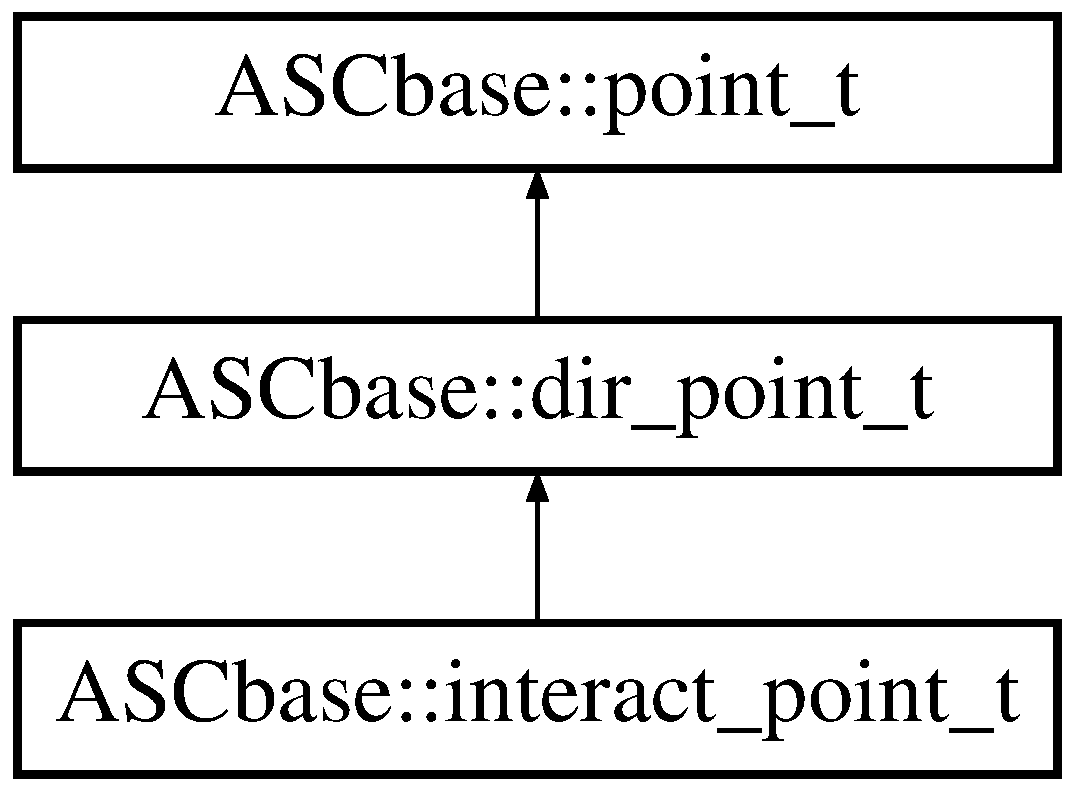
\includegraphics[height=3cm]{classASCbase_1_1interact__point__t}
\end{center}
\end{figure}
\subsection*{Public Member Functions}
\begin{CompactItemize}
\item 
\textbf{interact\_\-point\_\-t} (alloc\_\-t a=ALLOC\_\-POSITION)\label{classASCbase_1_1interact__point__t_847336b4146fb570f5dbf56a0cd1d2dc}

\item 
\textbf{interact\_\-point\_\-t} (const \bf{interact\_\-point\_\-t} \&p)\label{classASCbase_1_1interact__point__t_2d6a71e803d863c51a4fbd9d141c563c}

\item 
const \bf{interact\_\-point\_\-t} \& \textbf{operator=} (const \bf{interact\_\-point\_\-t} \&p)\label{classASCbase_1_1interact__point__t_b4f20ff04e85bf54b0ef6652ff899c04}

\end{CompactItemize}
\subsection*{Static Public Member Functions}
\begin{CompactItemize}
\item 
static bool \textbf{cmp} (const \bf{interact\_\-point\_\-t} \&A, const \bf{interact\_\-point\_\-t} \&B)\label{classASCbase_1_1interact__point__t_422857df1c11412c9c2b750f9d2d3ee2}

\end{CompactItemize}
\subsection*{Public Attributes}
\begin{CompactItemize}
\item 
interaction\-Type \bf{act\_\-type}\label{classASCbase_1_1interact__point__t_63eee3d009abf146282a6a8bf73bbaec}

\begin{CompactList}\small\item\em Interaction type of the points. \item\end{CompactList}\end{CompactItemize}
\subsection*{Private Member Functions}
\begin{CompactItemize}
\item 
void \textbf{do\_\-copy} (const \bf{interact\_\-point\_\-t} \&p)\label{classASCbase_1_1interact__point__t_01ba09e2cc58d89156b62a2398e24de1}

\end{CompactItemize}


\subsection{Detailed Description}
Interactions points. 



The documentation for this class was generated from the following file:\begin{CompactItemize}
\item 
interact\_\-point\_\-t.H\end{CompactItemize}
